\documentclass[fleqn, a4paper. 12pt]{ltjsarticle} 
% following is the compile command (以下のコマンドでコンパイル可能)
% $ lualatex guidance.tex 
% you need to install texlive to execute the above.(texlive を入れる必要がある.)
\usepackage{amsmath,txfonts}
\usepackage{amssymb}
\usepackage{url}
\usepackage{subcaption}
\usepackage[margin=31mm]{geometry}
\usepackage{graphicx}
\usepackage{listings}


\begin{document}
\begin{titlepage}
      \begin{center}
      {
      \Huge 2023年度\\言語処理 課題}
      
      \vspace{4cm}
             {\Huge 言語処理\\
               実験レポート\\}
             \vspace{4cm}
                    {\large 提出日:2024年2月7日(水)\\}
                    
                    {\large 学修番号:22140003\\氏名:佐倉仙汰郎}
    \end{center}  
  \end{titlepage}

  \section{課題1}
  \begin{figure}[h]
    \centering
    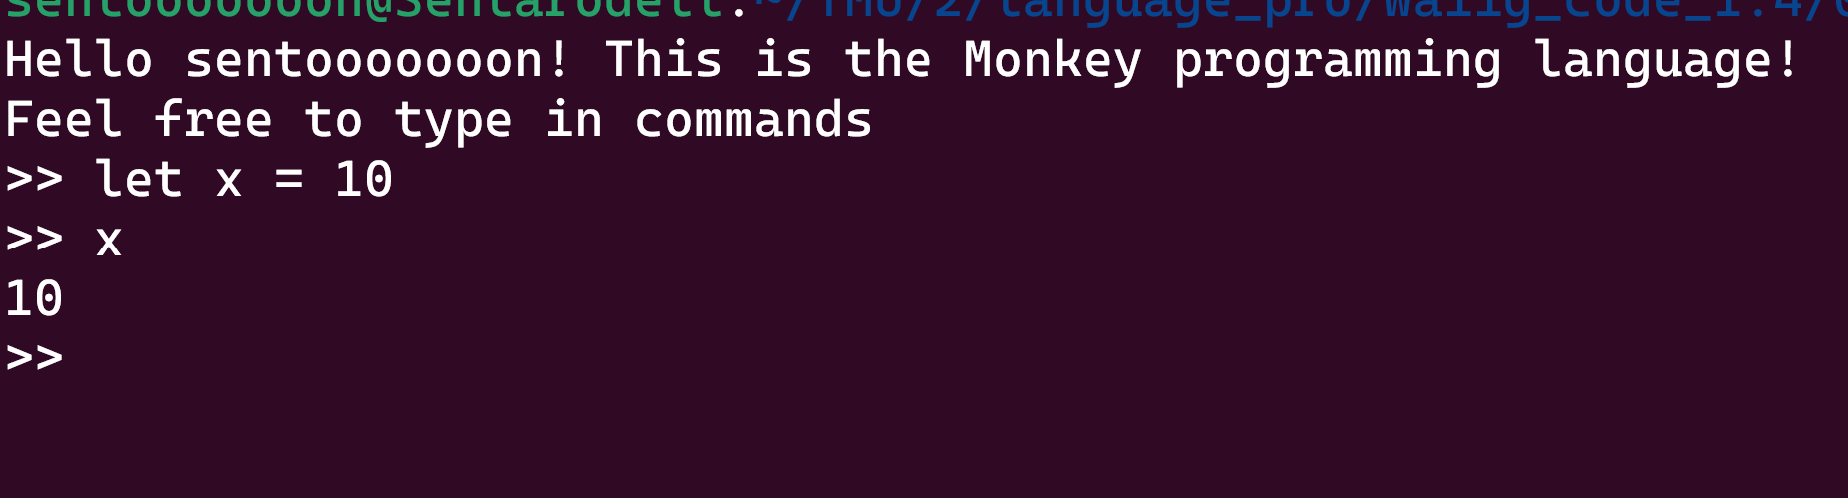
\includegraphics[width=0.5\linewidth]{images/2/1.png}
    \label{fig:1}
    \caption{変数の宣言}
\end{figure}

\section{課題2}
\begin{figure}[h]
    \centering
    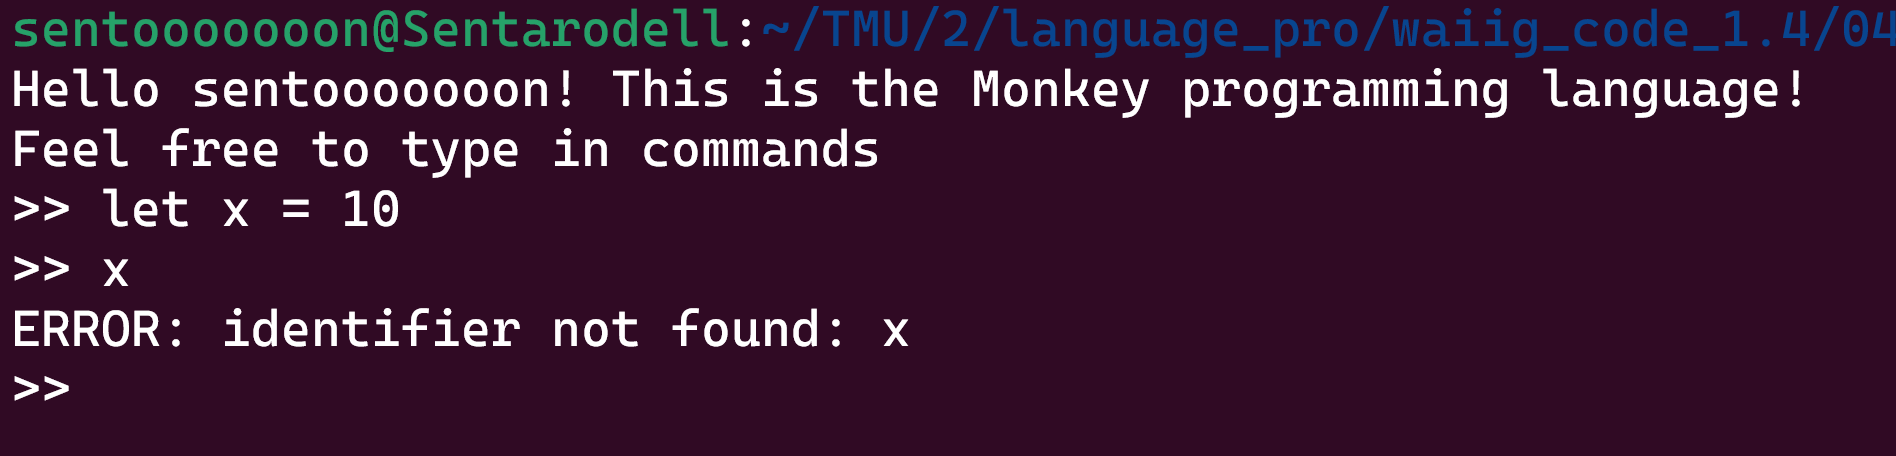
\includegraphics[width=0.5\linewidth]{images/2/2.png}
    \label{fig:2}
    \caption{Environment 型変数の定義を for ループの中に移動}
\end{figure}
\begin{figure}[h]
    \centering
    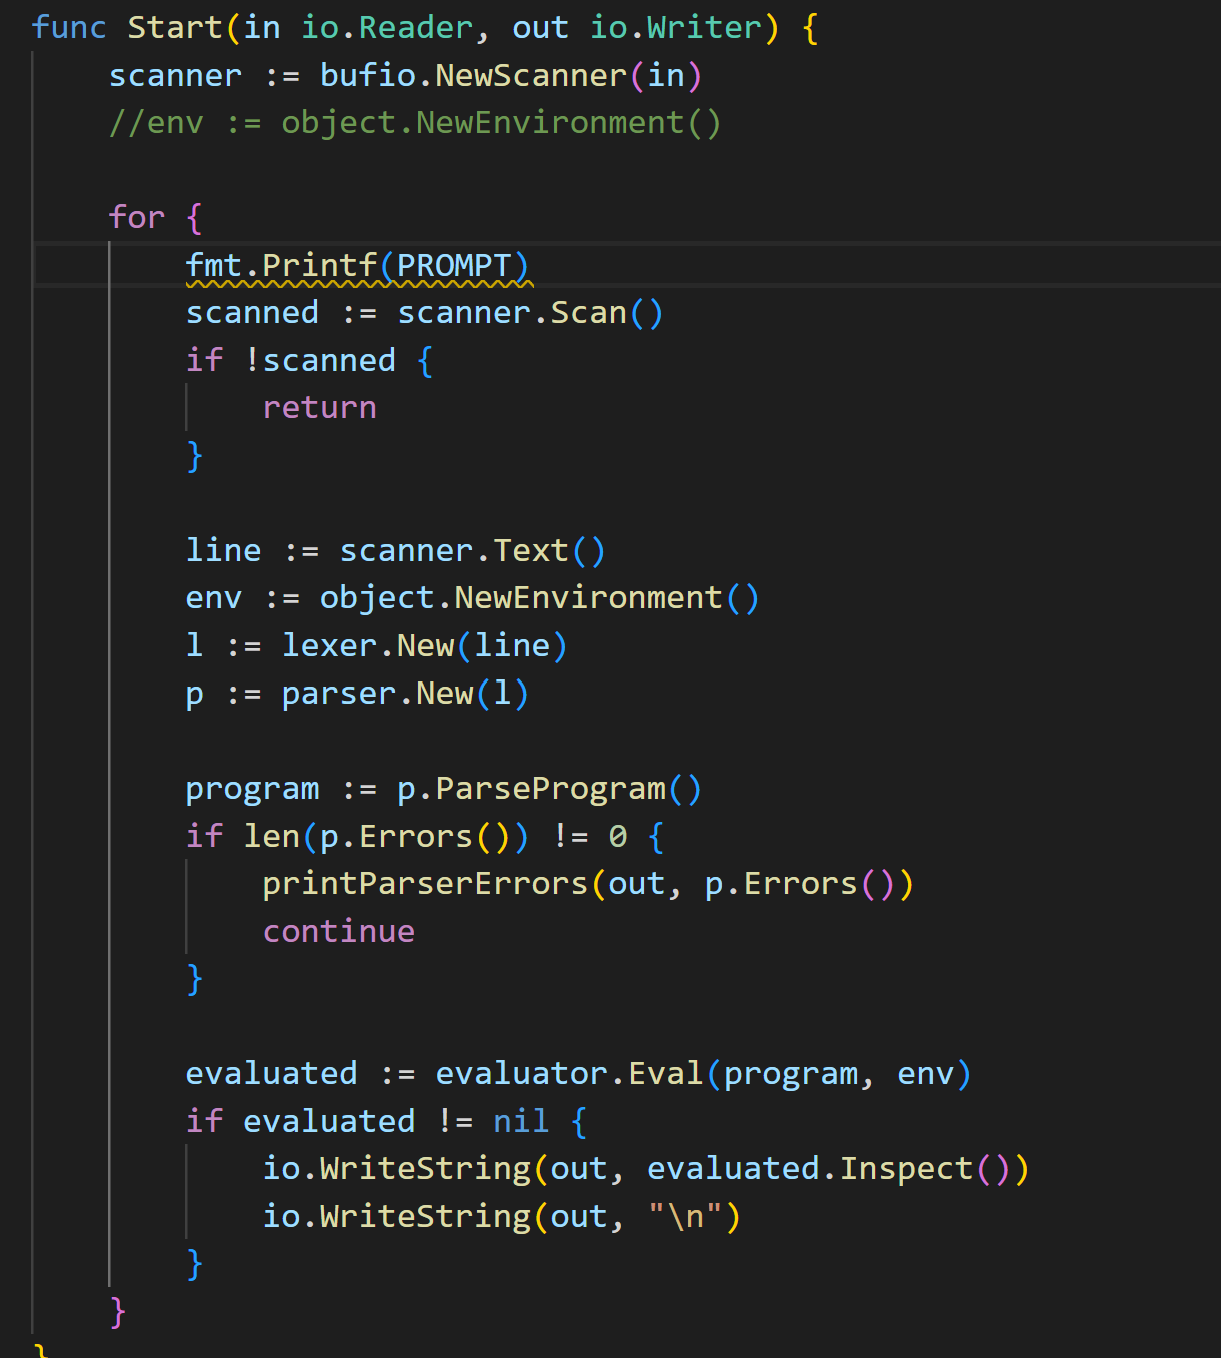
\includegraphics[width=0.5\linewidth]{images/2/2_repl.png}
    \label{fig:repl2}
    \caption{repl/repl.go で変更したコード}
\end{figure}

Environment 型変数の定義を for ループの中に移動することで、毎回新しい環境が生成される.
新しい環境が作られるときに、保持されていた変数がリセットされてしまうため、identifier not found となる.
\newpage

\section{課題3}
\begin{figure}[h]
    \centering
    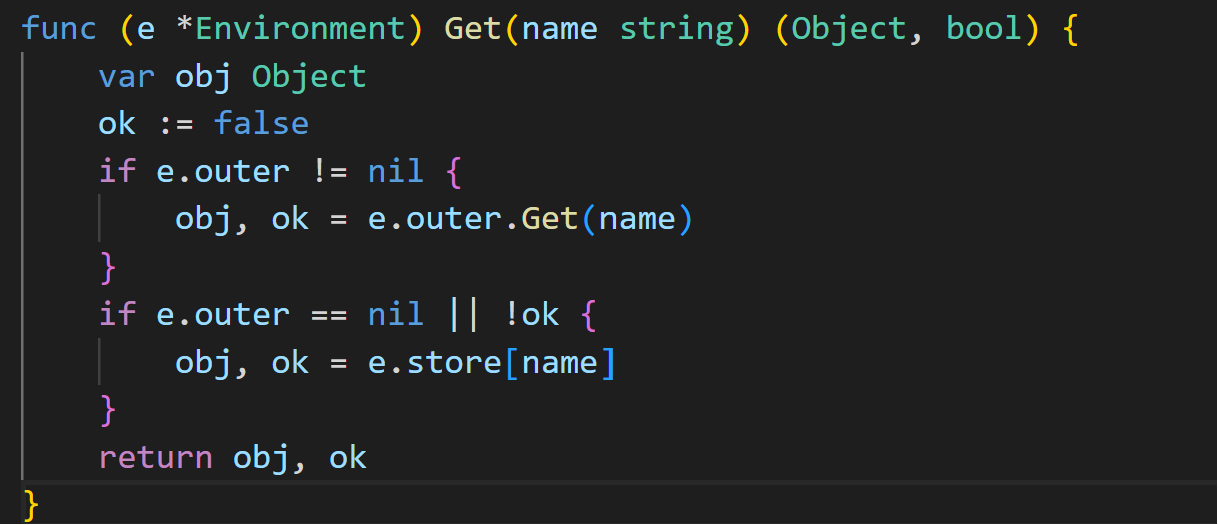
\includegraphics[width=0.5\linewidth]{images/2/3_env.png}
    \label{fig:env_3}
    \caption{object/environment.go で変更したコード}
\end{figure}
\begin{figure}[h]
    \centering
    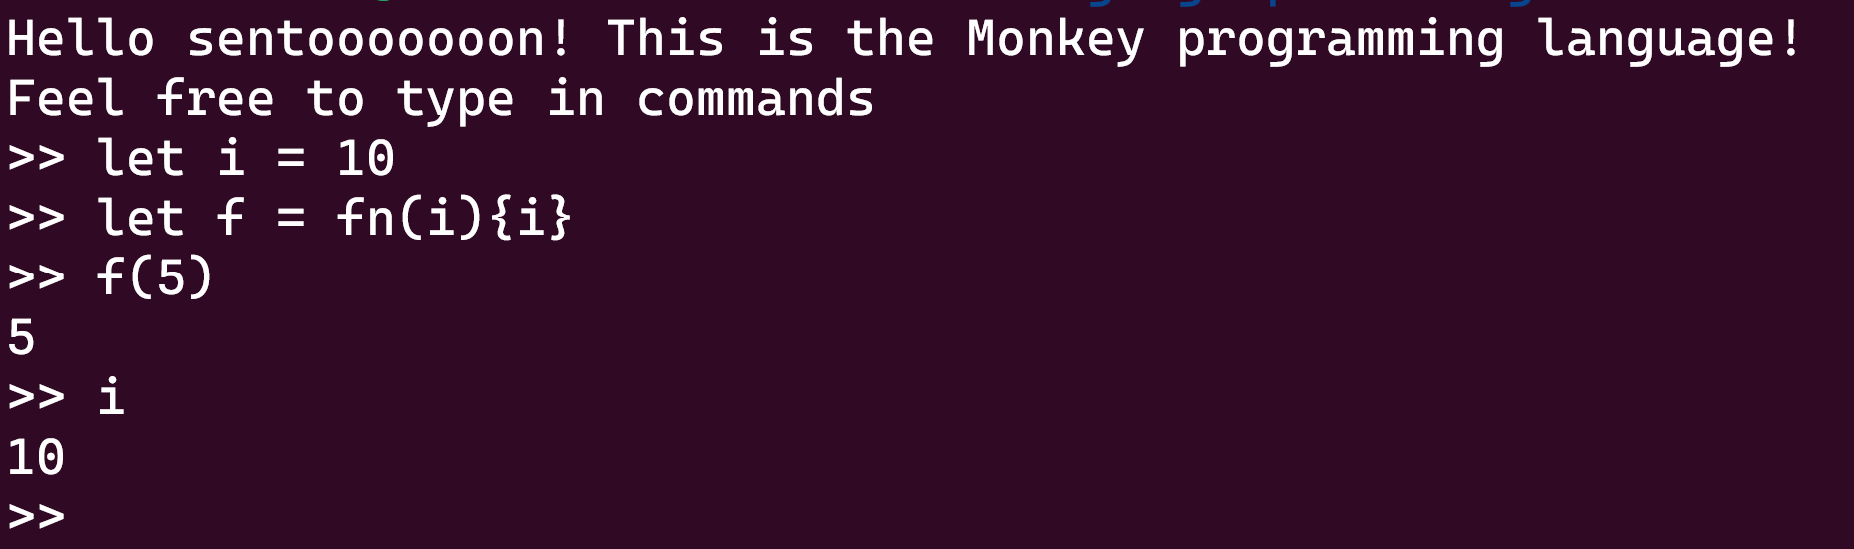
\includegraphics[width=0.5\linewidth]{images/2/3_before.png}
    \label{fig:3_before}
    \caption{変更前の結果}
\end{figure}
\begin{figure}[h]
    \centering
    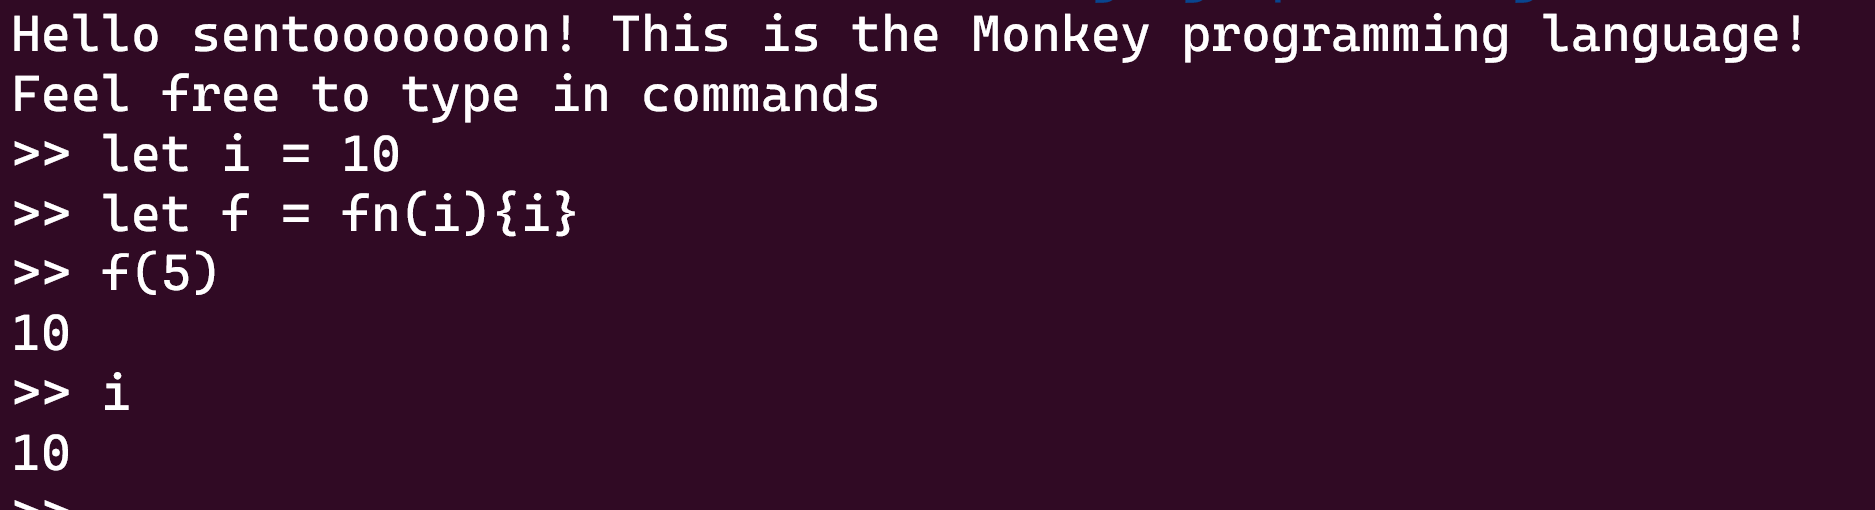
\includegraphics[width=0.5\linewidth]{images/2/3_after.png}
    \caption{変更後の結果}
    \label{fig:3_after}
\end{figure}

let x = 10 ではxという変数に10が代入されている.
また、 let f = fn(i){i} では引数をそのまま返す関数fが定義された.
変更後のプログラムでは、関数 f の中で変数 i を参照しているときに、i を現在の環境ではなく外部環境から取得するようになる.
そのため、f(5) を実行すると、関数 f 内の i が外部環境から取得され、その値である10が返されることになり図 \ref{fig:3_after} ような結果が得られる.

\section{課題4}
\begin{lstlisting}
    >> let newAdder = fn(x){fn(y){x+y}};
    >> let addTwo = newAdder(2);
    >> let addThree = newAdder(3);
    >> addThree
    fn(y) {
    (x + y)
    }
    >> addTwo
    fn(y) {
    (x + y)
    }
    \end{lstlisting}
    まず newAdder 関数はxとyを加算したものを返す関数として定義されている.
    let addTwo = newAdder(2); ではnewAdderのxに2が代入されたものとして定義されており,let addThree = newAdder(3);も同様にxに3が代入されている.
    したがって、addTwo と addThree は、newAdder が返す同一の関数リテラルを参照しており、そのために同じ関数リテラルが表示される.\\
    \begin{lstlisting}
        >> addTwo(0)
        2
        >> addThree(0)
        3
    \end{lstlisting}
    ここでは二回目に関数を呼び出すことで、addTwo(0)ではyに0がaddThree(0)でもyに0が代入されている.
    addTwoではx = 2,y = 0としてnewAdderが呼び出されるので、2 + 0 = 2 として結果が出力され、これはaddThreeでも同様である.
    以上の理由からこのような結果をえる.


\end{document}